\chapter{Appendix}

\section{Iterator Classes}
\label{sec:iterators}

\definecolor{CPPLight}  {HTML} {686868}
\definecolor{CPPSteel}  {HTML} {888888}
\definecolor{CPPDark}   {HTML} {262626}
\definecolor{CPPBlue}   {HTML} {4172A3}
\definecolor{CPPGreen}  {HTML} {487818}
\definecolor{CPPBrown}  {HTML} {A07040}
\definecolor{CPPRed}    {HTML} {AD4D3A}
\definecolor{CPPViolet} {HTML} {7040A0}
\definecolor{CPPGray}  {HTML} {B8B8B8}
\lstset{
    basicstyle=\fontfamily{pcr}\selectfont\tiny,
    columns=fixed,       
    numbers=left,                                        
    frame=none,                                          
    backgroundcolor=\color[RGB]{245,245,244},            
    keywordstyle=\color[RGB]{40,40,255},                 
    numberstyle=\tiny\color{darkgray},           
    commentstyle=\it\color[RGB]{0,96,96},                
    stringstyle=\rmfamily\slshape\color[RGB]{128,0,0},   
    showstringspaces=false,                              
    language=c++,                                        
    morekeywords={alignas,continute,friend,register,true,alignof,decltype,goto,
    reinterpret_cast,try,asm,defult,if,return,typedef,auto,delete,inline,short,
    typeid,bool,do,int,signed,typename,break,double,long,sizeof,union,case,
    dynamic_cast,mutable,static,unsigned,catch,else,namespace,static_assert,using,
    char,enum,new,static_cast,virtual,char16_t,char32_t,explict,noexcept,struct,
    void,export,nullptr,switch,volatile,class,extern,operator,template,wchar_t,
    const,false,private,this,while,constexpr,float,protected,thread_local,
    const_cast,for,public,throw,std},
    emph={map,set,multimap,multiset,unordered_map,unordered_set,
    unordered_multiset,unordered_multimap,vector,string,list,deque,
    array,stack,forwared_list,iostream,memory,shared_ptr,unique_ptr,
    random,bitset,ostream,istream,cout,cin,endl,move,default_random_engine,
    uniform_int_distribution,iterator,algorithm,functional,bing,numeric,},
    emphstyle=\color{CPPViolet}, 
}

\begin{figure*}[h!]
  \begin{minipage}{0.5\textwidth}
    \begin{lstlisting}[label={lst:table_iterator},caption={Table Iterator base class}]
      class table_iterator
      {
      protected:
        WT_CURSOR *cursor = nullptr;
        WT_SESSION *session = nullptr;
        bool is_first = true;
        bool has_next = true;
      
      public:
      table_iterator() = default;
      virtual ~table_iterator() = default;
      [[nodiscard]] bool has_more() const { return has_next; };
      virtual void reset()
      {
          cursor->reset(cursor);
          is_first = true;
          has_next = true;
      }
      void close() { cursor->close(cursor); }
      };
    \end{lstlisting}
  \end{minipage}
  \begin{minipage}{0.5\textwidth}
    \centering
    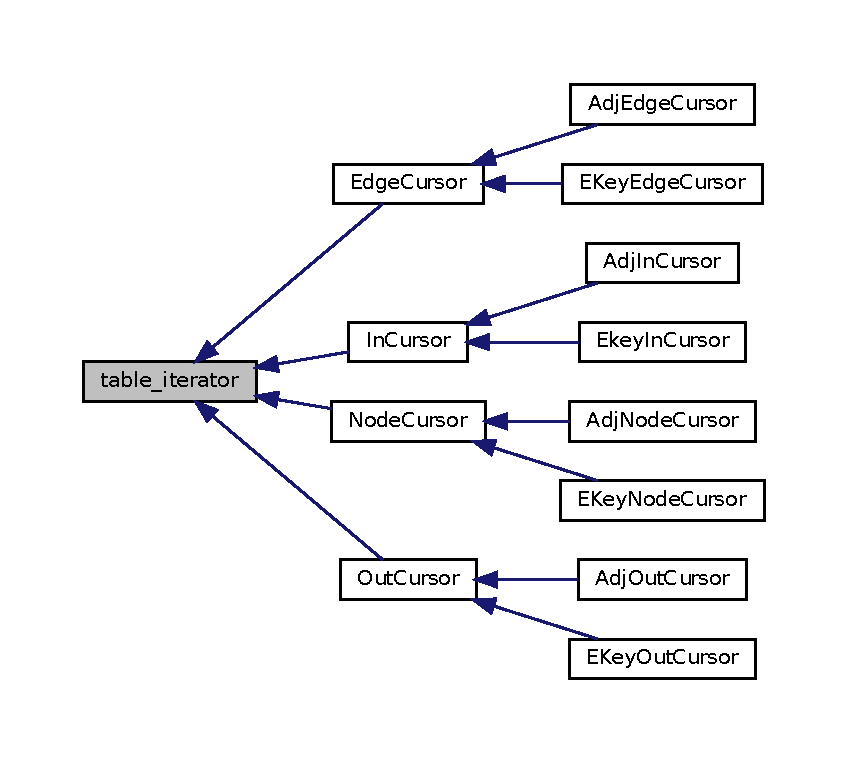
\includegraphics[scale=0.5]{content/fig/appendix/iterator_inherit_graph.pdf}
    \caption{Inheritance diagram for the iterator classes}
    \label{fig:iterator_diagram}
  \end{minipage}
\end{figure*}


\begin{lstlisting}[label={lst:pagerank_graphapi}, caption={GAPBS PageRank kernel modified to use~\api{}}]
  pvector<ScoreT> pagerank(GraphEngine& graph_engine,
                         int thread_num,
                         int max_iters,
                         node_id_t num_nodes,
                         node_id_t max_node_id,
                         double epsilon = 0)
{
    pvector<ScoreT> src(max_node_id, 0);
    pvector<ScoreT> dst(max_node_id, 1 / num_nodes);
    pvector<node_id_t> deg(max_node_id, 0);

#pragma omp parallel for
    for (int i = 0; i < thread_num; i++)
    {
        GraphBase* graph = graph_engine.create_graph_handle();
        NodeCursor* node_cursor = graph->get_node_iter();
        node_cursor->set_key_range(graph_engine.get_key_range(i));

        node found = {0};
        node_cursor->next(&found);

        while (found.id != -1)
        {
            deg[found.id] = found.out_degree;
            node_cursor->next(&found);
        }
        node_cursor->close();
        graph->close(false);
    }

    for (int iter = 0; iter < max_iters; iter++)
    {
        double error = 0;
#pragma omp parallel for reduction(+ : error)
        for (int i = 0; i < thread_num; i++)
        {
            GraphBase* graph = graph_engine.create_graph_handle();
            InCursor* in_cursor = graph->get_innbd_iter();
            in_cursor->set_key_range(graph_engine.get_key_range(i));

            adjlist found;
            in_cursor->next(&found);

            while (found.node_id != -1)
            {
                ScoreT incoming_total = 0;
                for (node_id_t v : found.edgelist)
                {
                    incoming_total += src[v];
                }

                ScoreT old_score = dst[found.node_id];
                dst[found.node_id] =
                    (1 - kDamp) / num_nodes + kDamp * incoming_total;
                error += fabs(dst[found.node_id] - old_score);
                src[found.node_id] = dst[found.node_id] / deg[found.node_id];

                in_cursor->next(&found);
            }

            in_cursor->close();
            graph->close(false);
        }
        printf(" %2d    %lf\n", iter, error);
        if (error < epsilon) break;
    }
    return dst;
}
\end{lstlisting}